\documentclass[a4paper]{article}

\usepackage[pdftex]{graphicx}
\usepackage{amsmath}
\usepackage{amsfonts,amssymb} \usepackage{amsthm} % for new theorem
\usepackage{thmtools} \usepackage{mathtools}
\usepackage[colorlinks=true]{hyperref} \usepackage{epstopdf} \usepackage{url}

\usepackage[font=footnotesize]{caption}%needed for subcaption
\usepackage[font+=small]{subcaption}

\usepackage{units} \usepackage{booktabs} %for table rulers \usepackage{tabulary}

\setlength{\parindent}{0pt}

\usepackage[utf8]{inputenc} \DeclareMathOperator*{\argmin}{arg\,min}

\graphicspath{{figs/}} \usepackage[top=1in, bottom=1in, left=1in,
  right=1in]{geometry}

\title{16831 Lab 2: Online learning}

\author{Mike Phillips, mlphilli \and Siddharth Swaminathan, sswamin1 \and
  Abhijeet Tallavajhula, atallav1}

\begin{document}
\maketitle

\section{Algorithms}
We implemented the following algorithms:
\begin{itemize}
\item One-vs-all logistic regression (OVA LR).
\item Multiclass logistic regression (Multi LR).
\item One-vs-all exponentiated gradient descent (OVA Exp). \\
  The one-vs-all
  algorithms train $L$ one-vs-all classifiers (one for each class)
  independently. During test, the classifier with maximum `confidence'
  (probability or margin) is chosen as the predicted class.
\item Multiclass exponentiated gradient descent (Multi Exp). \\
  This algorithm uses
  the same loss as SVM. The difference is in the update step. Each dimension of
  the weight vector undergoes a multiplicative update. 
\item Multiclass SVM (SVM).
\item Kernel multiclass SVM (Kernel SVM). \\
  Implemented with an RBF kernel.
\end{itemize}

We trained on the scene \texttt{oakland\_part3\_am\_rf.node\_features} and
tested on the scene \\ \texttt{oakland\_part3\_an\_rf.node\_features}. Training
was `online' in that weights were updated after seeing each
instance. 

Other choices to talk about:
\begin{itemize}
\item Randomizing made a beeg dipharence.
\item Balancing of data.
\item Number of passes through data.
\item Whitening.
\end{itemize}

\section{Parameter selection}
The learning rate was chosen in all cases $\propto 1/\sqrt{t}$. All classes have
regularization constant as a hyperparameter. In addition, Kernel SVM has kernel
width and history size (of kernels) as hyperparameters.

\section{Results}
All implementation was in C++. Runtimes are shown in Table \ref{table:runtimes}.

\begin{table}[h]
\centering
\begin{tabular}{|l|l|l|l|l|l|l|}
\hline
& OVA LR & Multi LR & OVA Exp & Multi Exp & SVM & Kernel SVM \\ \hline
Single pass training (CPU s) & 0.34 & 1.75 & 0.36 & 2.84 & 1.18 &  \\ \hline
Test (CPU s) & 0.04 & 0.07 & 0.07 & 0.07 & 0.04 &  \\ \hline
\end{tabular}
\caption{Runtimes}
\label{table:runtimes}
\end{table}

\begin{table}[h]
\centering
\begin{tabular}{|l|l|l|l|l|l|}
\hline
 & Veg & Wire & Pole & Ground & Facade \\
\hline
OVA LR &  &  &  &  &  \\
\hline
Multi LR &  &  &  &  &  \\
\hline
OVA Exp &  &  &  &  &  \\
\hline
Multi Exp &  &  &  &  &  \\
\hline
SVM &  &  &  &  &  \\
\hline
Kernel SVM &  &  &  &  & \\
\hline
\end{tabular}
\caption{Per-class accuracy on training data.}
\end{table}

\begin{table}[h]
\centering
\begin{tabular}{|l|l|l|l|l|l|}
\hline
 & Veg & Wire & Pole & Ground & Facade \\
\hline
OVA LR &  &  &  &  &  \\
\hline
Multi LR &  &  &  &  &  \\
\hline
OVA Exp &  &  &  &  &  \\
\hline
Multi Exp &  &  &  &  &  \\
\hline
SVM &  &  &  &  &  \\
\hline
Kernel SVM &  &  &  &  & \\
\hline
\end{tabular}
\caption{Per-class accuracy on test data.}
\end{table}

\subsection{Dataset Collection}
\begin{figure}[!htp]
  \centering
  \begin{subfigure}[b]{.3\linewidth}
    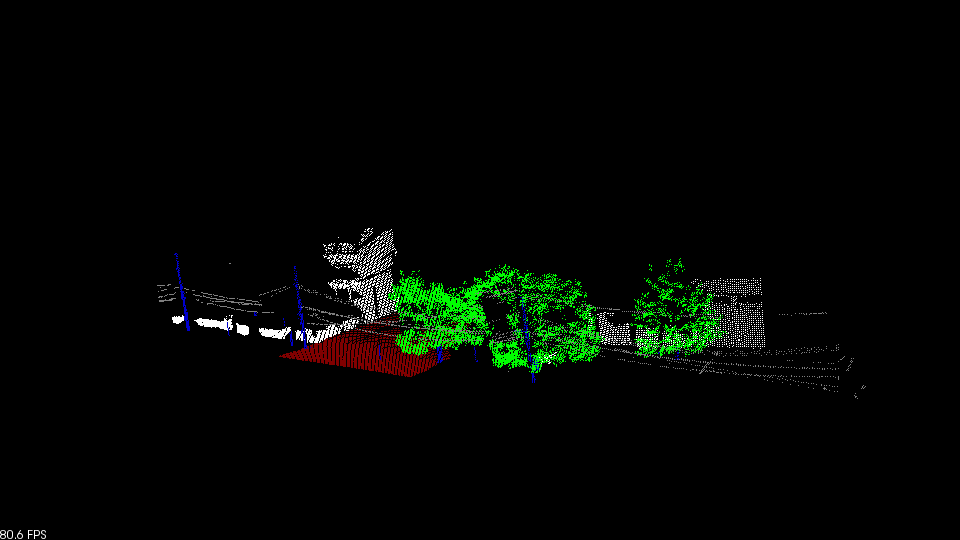
\includegraphics[width=\textwidth]{ground_truth_test.png}
        \caption{Ground truth}
  \end{subfigure} \quad
  \begin{subfigure}[b]{.3\linewidth}
    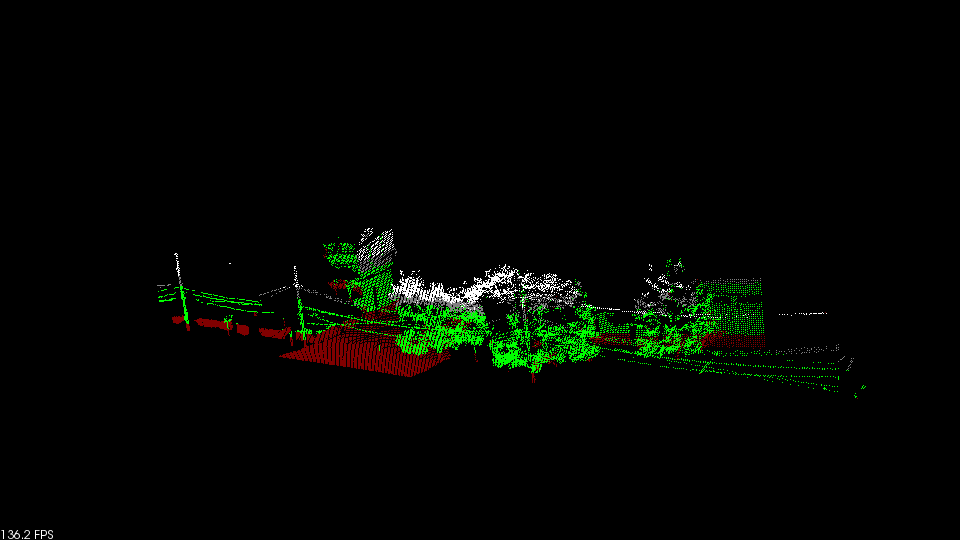
\includegraphics[width=\textwidth]{logistic_test.png}
        \caption{OVA LR}
  \end{subfigure}\quad
  \begin{subfigure}[b]{.3\linewidth}
    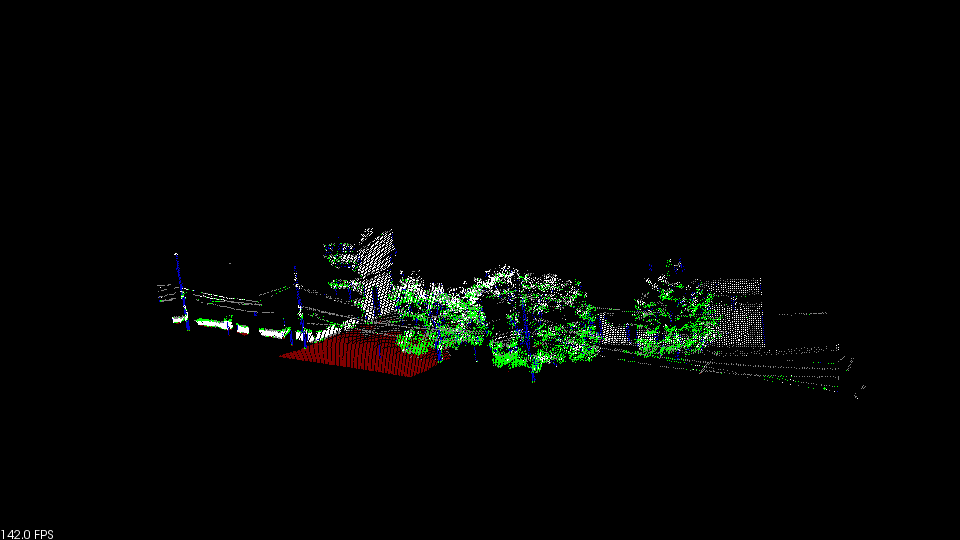
\includegraphics[width=\textwidth]{multilog_test.png}
        \caption{Multi LR}
    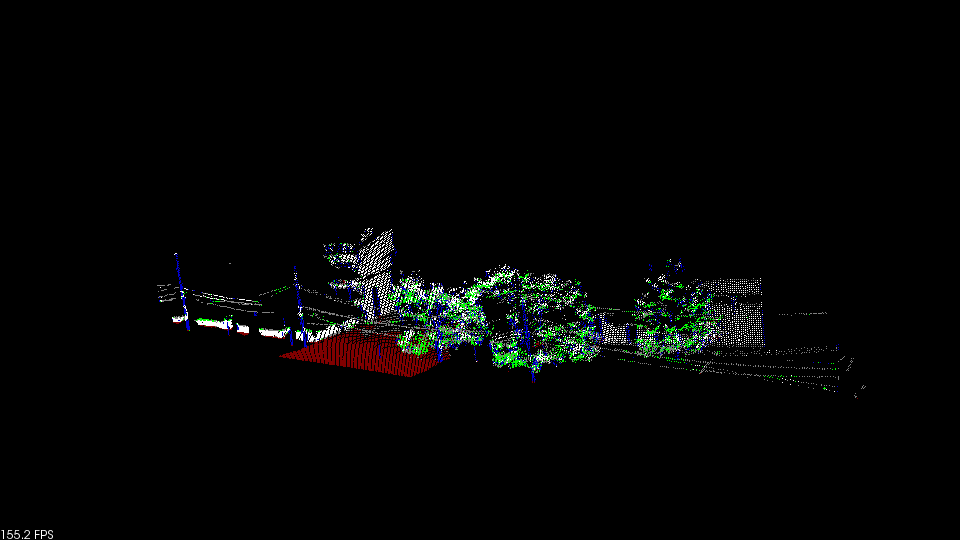
\includegraphics[width=\textwidth]{exp_test.png}
        \caption{OVA Exp}
  \end{subfigure} \quad
  \begin{subfigure}[b]{.3\linewidth}
    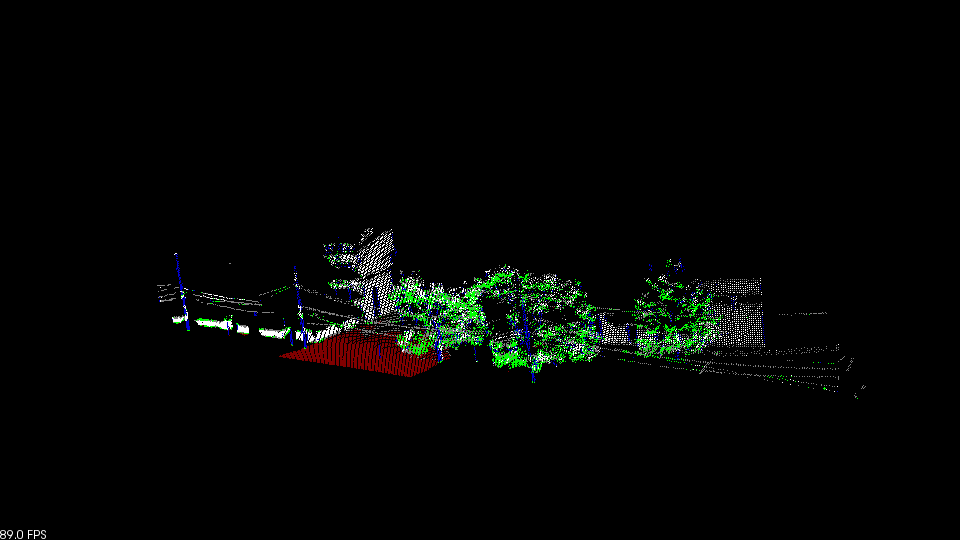
\includegraphics[width=\textwidth]{multiexp_test.png}
        \caption{Multi Exp}
  \end{subfigure}\quad
  \begin{subfigure}[b]{.3\linewidth}
    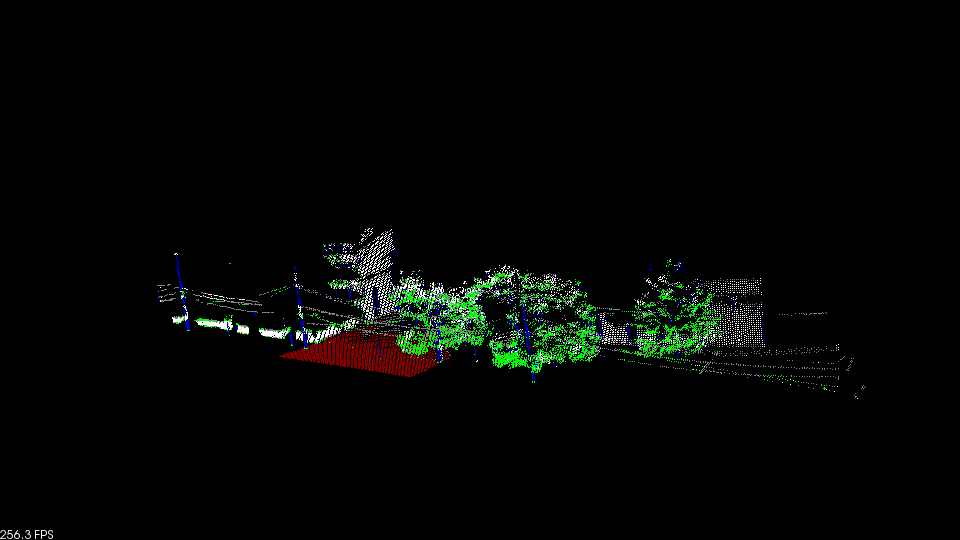
\includegraphics[width=\textwidth]{svm_test.png}
        \caption{SVM}

  \end{subfigure}\\
  \caption{\label{fig:viz_test} 
  }
\end{figure}


\section{Future Work}

\begin{thebibliography}{10}
\end{thebibliography}
\end{document}













